\documentclass[a4paper,12pt]{article}

\usepackage{fancyhdr}
\usepackage{graphicx}
\usepackage{listings}
\usepackage{extramarks}
\usepackage{courier}
\usepackage{geometry}
\usepackage{hyperref}

\geometry{lmargin=1in,rmargin=1in, bmargin=1in}

\pagestyle{fancy}
\lhead{James Palmer}
\chead{\large \bfseries ENEE499 Mid-Semester Report}
\rhead{\today}


\setlength{\parindent}{0em}
\setlength{\parskip}{0.5em}

\lstloadlanguages{C++}
\lstset{language=C++,
        frame=single,
        basicstyle=\small\ttfamily,
}

\begin{document}

\title{``Spider Square'' Robot Mid-Semester Project Report}
\author{James Palmer}

\section*{C++ and OpenCV}
We have decided to use C++ as the primary language for this project, for its
extensive OpenCV (Open Source Computer Vision Library) API support, ability to
interface with any stylus driver board (USB or GPIO), and ability to compile
and optimize code for different platforms, ARM or x86-64. Since speed is vital,
the ability to have a compiler optimize our code ahead of time should lead to
better runtimes.

I compiled OpenCV 3.1.0 for my x86-64 Linux workstation, created a GitHub
repository, and created a simple Makefile-based build system for our code. I
then worked on two different OpenCV side projects, reading frames from
pre-recorded gameplay and parsing them, and reading frames from a webcam.

\subsection*{Parsing Pre-Recorded Gameplay}
I played the game on my phone and recorded the screen to a video file that I 
could then replay in OpenCV using the provided \texttt{VideoCapture} class. The
image below shows one processed frame. It gathers information about the player
location and the obstacles forward of the player. \\

\centerline{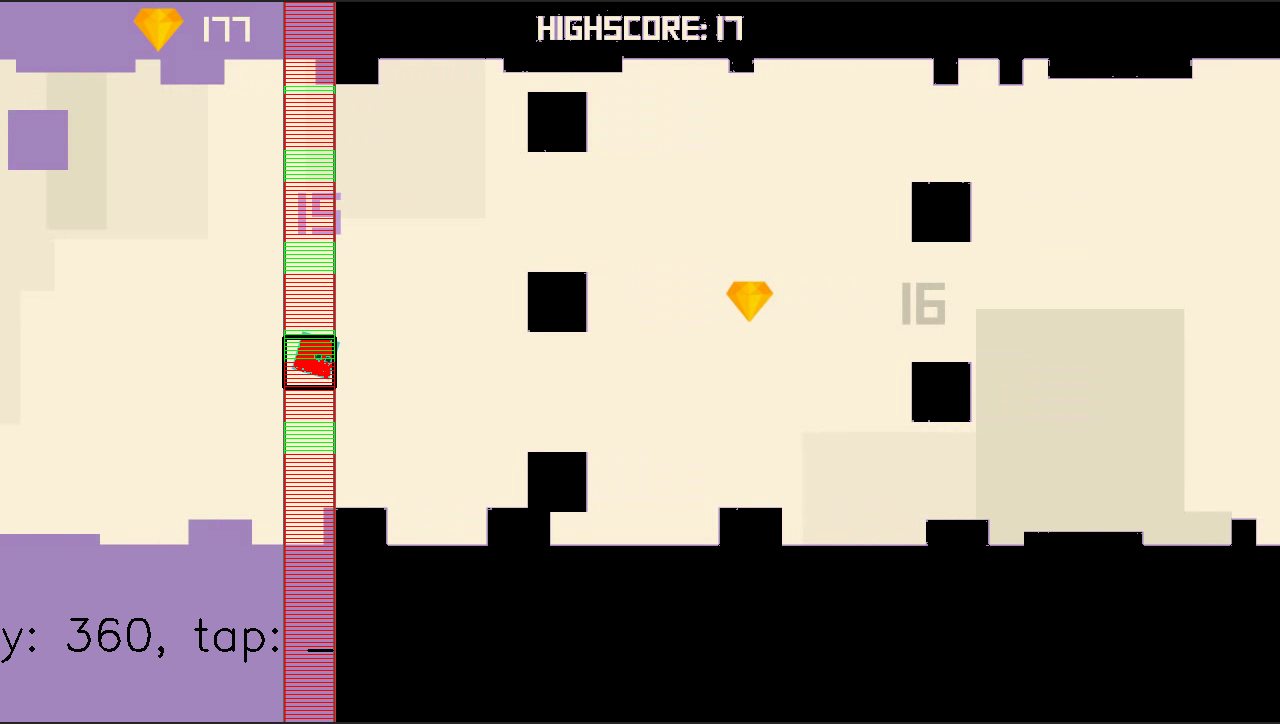
\includegraphics[height=3.2in]{f1.png}}

Since the player remains in the same horiziontal position at all times and does
not change color (unlike the obstacles), finding the player within that column
of pixels is straightforward. I used the \texttt{inRange()} function to find
all the pixels that match the specific blue color of the player, which gives a
bitmask of all the pixels within the colum that match the player. The y position
is drawn to the screen for debugging purposes. This position will be one input
to our neural network.

Identifyting the obstacles is done by first determining the stage color, using
the \texttt{Mat.at()} function to sample the pixel at (0,0), since the
stage changes color as the player progresses but is always uniform on-screen.
Another mask is applied to the area to the right of the player that matches on
the stage color (shown in black above). By taking the average value at different
rows of pixels, it can be determined which rows contain an obstacle. These open
spaces, shown in green above, could be inputs to our neural network. We may
decide to use different inputs, like the X,Y coordinates of the closest 3
obstacles.

\subsection*{Webcam or Capture Device}

I also experimented reading input from a webcam, which is done pretty similarly
in OpenCV with a \texttt{VideoCapture} object. There is some very slight delay
between the camera and displaying the processed frame, but I need to
investigate further the source of the delay, as there are many: camera sensor,
USB bus, reading frame into memory, graphics draw time, and monitor pixel
delay.

I also have a PCI-based HDMI capture card that can be used to feed the phone's
screen directly into the controlling machine, although it would have to support
PCIe expansion cards, have the correct drivers, and use a phone that supports
MHL to output HDMI over its USB port. I have not tested the delay on this card
yet.

\section*{Neural Networks}

Haris and I have both done some preliminary readings on the literature on
artificial neural networks. We're likely going to start out with a simple
multilayer network, with one "hidden" layer of nodes, a few inputs, one output
(touch or not for that frame), and assignment of edge weights using the
gameplay recordings. The following figure demonstrates a network with a single
input, output, and hidden layer (and included bias units): \\

\centerline{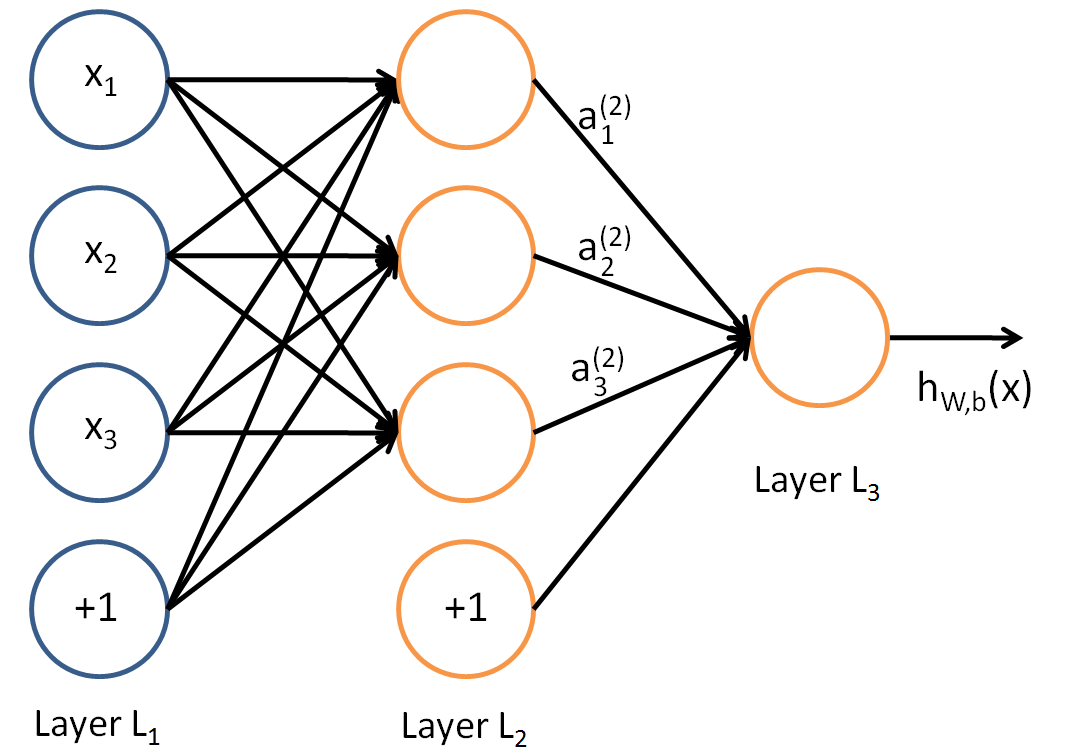
\includegraphics[height=2.5in]{f2.png}}
{\footnotesize Source: 
\url{http://ufldl.stanford.edu/tutorial/supervised/MultiLayerNeuralNetworks/}}

\end{document}
